% !TEX root=./adl.tex

% -----------------------------------------------------------------------
\begin{frame}{Pipeline Parallelism: Core Idea}

  Split the model's \emph{layers} across GPUs, forming a sequential \emphdef{pipeline}.

  \vspace{0.3em}
  \begin{columns}
    \begin{column}{0.52\textwidth}
      \begin{center}
      \begin{tikzpicture}[
        scale=0.65, transform shape,
        layer/.style={draw, rounded corners=2pt, minimum width=2.8cm, minimum height=0.38cm,
                      font=\scriptsize, inner sep=1pt},
        gpubox/.style={draw, rounded corners=4pt, inner sep=5pt, thick},
        arr/.style={->, thick, gray!70},
      ]
        % GPU 0 -- layers 1-4
        \node[layer, fill=blue!20]   (l1) at (0, 0)    {Layer 1};
        \node[layer, fill=blue!20]   (l2) at (0,-0.55) {Layer 2};
        \node[layer, fill=blue!20]   (l3) at (0,-1.10) {Layer 3};
        \node[layer, fill=blue!20]   (l4) at (0,-1.65) {Layer 4};
        \begin{pgfonlayer}{background}
          \node[gpubox, fill=blue!5, fit=(l1)(l2)(l3)(l4)] (g0) {};
        \end{pgfonlayer}
        \node[font=\scriptsize\bfseries, anchor=east, align=center] at ([xshift=-4pt]g0.west) {GPU 0\\Stage 1};

        % GPU 1 -- layers 5-8
        \node[layer, fill=green!20]  (l5) at (0,-3.35) {Layer 5};
        \node[layer, fill=green!20]  (l6) at (0,-3.90) {Layer 6};
        \node[layer, fill=green!20]  (l7) at (0,-4.45) {Layer 7};
        \node[layer, fill=green!20]  (l8) at (0,-5.00) {Layer 8};
        \begin{pgfonlayer}{background}
          \node[gpubox, fill=green!5, fit=(l5)(l6)(l7)(l8)] (g1) {};
        \end{pgfonlayer}
        \node[font=\scriptsize\bfseries, anchor=east, align=center] at ([xshift=-4pt]g1.west) {GPU 1\\Stage 2};

        % GPU 2 -- layers 9-12
        \node[layer, fill=orange!20] (l9)  at (0,-6.70) {Layer 9};
        \node[layer, fill=orange!20] (l10) at (0,-7.25) {Layer 10};
        \node[layer, fill=orange!20] (l11) at (0,-7.80) {Layer 11};
        \node[layer, fill=orange!20] (l12) at (0,-8.35) {Layer 12};
        \begin{pgfonlayer}{background}
          \node[gpubox, fill=orange!5, fit=(l9)(l10)(l11)(l12)] (g2) {};
        \end{pgfonlayer}
        \node[font=\scriptsize\bfseries, anchor=east, align=center] at ([xshift=-4pt]g2.west) {GPU 2\\Stage 3};

        % Arrows: activations between stages
        \draw[arr] (0,-1.90) -- (0,-3.10);
        \node[font=\tiny, text=gray, anchor=west] at (0.15,-2.50) {activations};
        \draw[arr] (0,-5.25) -- (0,-6.45);
        \node[font=\tiny, text=gray, anchor=west] at (0.15,-5.85) {activations};

        % Input / output
        \draw[arr] (0, 0.9) -- (0, 0.25);
        \node[font=\tiny, text=gray, anchor=west] at (0.15, 0.58) {input};
        \draw[arr] (0,-8.60) -- (0,-9.25);
        \node[font=\tiny, text=gray, anchor=west] at (0.15,-8.93) {output};
      \end{tikzpicture}
      \end{center}
    \end{column}
    \begin{column}{0.45\textwidth}
      \textbf{How it works}
      \begin{itemize}
        \item Partition $L$ layers into $p$ \emphdef{stages}
        \item Stage $i$ sits on GPU $i$
        \item Activations passed \emph{P2P} between stages
      \end{itemize}

      \vspace{0.2em}
      \textbf{Parameter memory}
      \begin{itemize}
        \item Each GPU stores $\frac{1}{p}$ of weights, gradients, optimizer states
        \item $\frac{16\Psi}{p}$ per GPU
      \end{itemize}

      \vspace{0.2em}
      \textbf{Activations NOT reduced!}
      \begin{itemize}
        \item $\frac{1}{p}$ layers per GPU, but $p$ in-flight micro-batches before backward
        \item $p \times \frac{\text{activs}}{p} = \text{activs}$
        \item Pipeline schedule artifact; details below
      \end{itemize}

      \vspace{0.2em}
      \textbf{Communication per micro-batch:}\par
      {\small $4 \cdot \text{seq} \cdot \text{mbs} \cdot h$ bytes (P2P)}
    \end{column}
  \end{columns}
\end{frame}

% -----------------------------------------------------------------------
\begin{frame}{The Pipeline Bubble}

  The fundamental challenge: GPUs sit \emph{idle} while waiting for activations from upstream stages.

  \vspace{0.3em}
  \begin{center}
  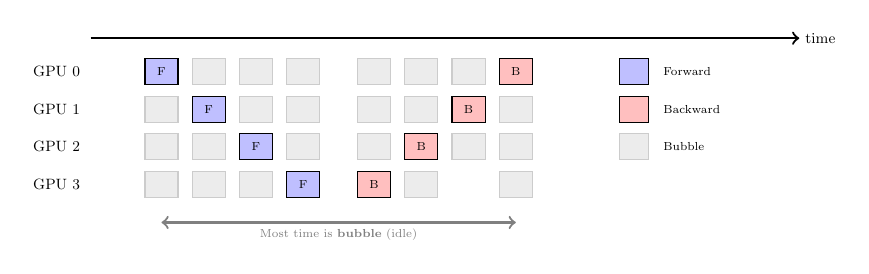
\begin{tikzpicture}[
    scale=0.60, transform shape,
    stage/.style={draw, minimum width=0.7cm, minimum height=0.55cm, font=\scriptsize, inner sep=1pt},
    fwd/.style={stage, fill=blue!25},
    bwd/.style={stage, fill=red!25},
    bubble/.style={stage, fill=gray!15, draw=gray!40},
  ]
    % Time axis
    \draw[->, thick] (-0.5, -0.3) -- (14.5, -0.3) node[right, font=\small] {time};
    % GPU labels
    \foreach \g in {0,1,2,3} {
      \node[font=\small, anchor=east] at (-0.6, -\g*0.8 - 1.0) {GPU \g};
    }
    % Naive pipeline: single micro-batch, 4 stages
    % Forward passes (sequential)
    \node[fwd] at (1.0, -1.0) {F};
    \node[bubble] at (1.0, -1.8) {};
    \node[bubble] at (1.0, -2.6) {};
    \node[bubble] at (1.0, -3.4) {};

    \node[bubble] at (2.0, -1.0) {};
    \node[fwd] at (2.0, -1.8) {F};
    \node[bubble] at (2.0, -2.6) {};
    \node[bubble] at (2.0, -3.4) {};

    \node[bubble] at (3.0, -1.0) {};
    \node[bubble] at (3.0, -1.8) {};
    \node[fwd] at (3.0, -2.6) {F};
    \node[bubble] at (3.0, -3.4) {};

    \node[bubble] at (4.0, -1.0) {};
    \node[bubble] at (4.0, -1.8) {};
    \node[bubble] at (4.0, -2.6) {};
    \node[fwd] at (4.0, -3.4) {F};

    % Backward passes (sequential, reverse)
    \node[bubble] at (5.5, -1.0) {};
    \node[bubble] at (5.5, -1.8) {};
    \node[bubble] at (5.5, -2.6) {};
    \node[bwd] at (5.5, -3.4) {B};

    \node[bubble] at (6.5, -1.0) {};
    \node[bubble] at (6.5, -1.8) {};
    \node[bwd] at (6.5, -2.6) {B};
    \node[bubble] at (6.5, -3.4) {};

    \node[bubble] at (7.5, -1.0) {};
    \node[bwd] at (7.5, -1.8) {B};
    \node[bubble] at (7.5, -1.8) {};
    \node[bubble] at (7.5, -2.6) {};

    \node[bwd] at (7.5, -1.8) {B};

    \node[bwd] at (8.5, -1.0) {B};
    \node[bubble] at (8.5, -1.8) {};
    \node[bubble] at (8.5, -2.6) {};
    \node[bubble] at (8.5, -3.4) {};

    % Legend
    \node[fwd, minimum width=0.6cm] at (11.0, -1.0) {};
    \node[font=\scriptsize, anchor=west] at (11.5, -1.0) {Forward};
    \node[bwd, minimum width=0.6cm] at (11.0, -1.8) {};
    \node[font=\scriptsize, anchor=west] at (11.5, -1.8) {Backward};
    \node[bubble, minimum width=0.6cm] at (11.0, -2.6) {};
    \node[font=\scriptsize, anchor=west] at (11.5, -2.6) {Bubble};
    % Bubble annotation
    \draw[<->, gray, thick] (1.0, -4.2) -- (8.5, -4.2);
    \node[font=\scriptsize, gray, below] at (4.75, -4.2) {Most time is \textbf{bubble} (idle)};
  \end{tikzpicture}
  \end{center}

  \vspace{0.2em}
  With a single micro-batch and $p$ stages, the \emphdef{bubble ratio} is:
  \[
    r_{\text{bubble}} = \frac{(p-1)(t_f + t_b)}{t_f + t_b} = p - 1
  \]
  where $t_f, t_b$ are forward/backward times per stage. \textbf{Catastrophic} for large $p$.

  \vspace{0.3em}
  \textbf{Solution:} Split each batch into $m$ \emphdef{micro-batches} and pipeline them $\Rightarrow$ multiple schedules.
\end{frame}

% -----------------------------------------------------------------------
\begin{frame}{Schedule 1: All-Forward-All-Backward (AFAB)}

  Also known as \emphdef{GPipe} schedule~\cite{huang2019gpipe}. Simplest pipeline schedule.

  \vspace{0.3em}
  \begin{center}
  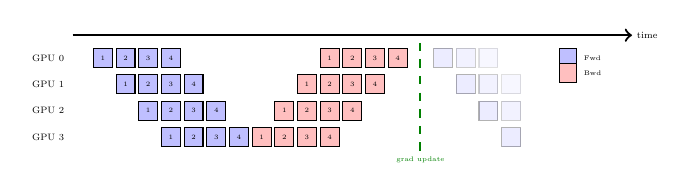
\begin{tikzpicture}[
    scale=0.48, transform shape,
    stage/.style={draw, minimum width=0.50cm, minimum height=0.50cm, font=\tiny, inner sep=1pt},
    fwd/.style={stage, fill=blue!25},
    bwd/.style={stage, fill=red!25},
    bubble/.style={stage, fill=gray!12, draw=gray!35},
  ]
    \def\s{0.60}% step size
    \draw[->, thick] (-0.3, -0.1) -- (14.5, -0.1) node[right, font=\scriptsize] {time};
    \foreach \g in {0,1,2,3} {
      \node[font=\scriptsize, anchor=east] at (-0.4, -\g*0.7 - 0.7) {GPU \g};
    }
    % Forward passes: GPU g starts micro-batch m at time g+m
    % m=4 micro-batches, p=4 GPUs
    \foreach \m [count=\mi from 0] in {1,2,3,4} {
      \foreach \g in {0,1,2,3} {
        \pgfmathtruncatemacro{\t}{\mi + \g}
        \pgfmathsetmacro{\y}{-\g*0.7 - 0.7}
        \node[fwd] at (\t*\s + 0.5, \y) {\m};
      }
    }
    % Backward passes: start at time slot 7 (= last fwd slot 6 + 1)
    \foreach \m [count=\mi from 0] in {1,2,3,4} {
      \foreach \g [count=\gi from 0] in {3,2,1,0} {
        \pgfmathtruncatemacro{\t}{\mi + \gi + 7}
        \pgfmathsetmacro{\y}{-\g*0.7 - 0.7}
        \node[bwd] at (\t*\s + 0.5, \y) {\m};
      }
    }
    % Gradient update: vertical bar after last backward (time slot 14)
    \draw[thick, green!50!black, dashed] (14*\s+0.5, -0.3) -- (14*\s+0.5, -3.2)
      node[below, font=\tiny, text=green!50!black] {grad update};
    % Next cycle: faded forward passes starting at time slot 15
    \foreach \col [count=\ci from 0] in {0.30, 0.20, 0.12} {
      \foreach \g in {0,1,2,3} {
        \pgfmathtruncatemacro{\t}{15 + \ci + \g}
        \pgfmathsetmacro{\y}{-\g*0.7 - 0.7}
        \ifnum\t<19
          \node[fwd, opacity=\col] at (\t*\s + 0.5, \y) {};
        \fi
      }
    }
    % Legend
    \node[fwd, minimum width=0.45cm] at (12.8, -0.7) {};
    \node[font=\tiny, anchor=west] at (13.1, -0.7) {Fwd};
    \node[bwd, minimum width=0.45cm] at (12.8, -1.1) {};
    \node[font=\tiny, anchor=west] at (13.1, -1.1) {Bwd};
  \end{tikzpicture}
  \end{center}

  \vspace{0.2em}
  \begin{columns}
    \begin{column}{0.48\textwidth}
      \textbf{Algorithm:}
      \begin{enumerate}
        \item Run all $m$ forward passes through the pipeline
        \item Then run all $m$ backward passes
        \item Optimizer step
      \end{enumerate}

      \vspace{0.3em}
      \textbf{Bubble ratio with $m$ micro-batches:}
      \[
        r_{\text{bubble}} = \frac{p - 1}{m}
      \]
      Increasing $m$ shrinks the bubble.
    \end{column}
    \begin{column}{0.48\textwidth}
      \textbf{Pros:}
      \begin{itemize}
        \item Simplest to implement
        \item Clean separation of fwd/bwd phases
      \end{itemize}

      \vspace{0.3em}
      \textbf{Cons:}
      \begin{itemize}
        \item Must store activations for \emph{all} $m$ micro-batches until backward phase
        \item Activation memory scales as $O(m)$: \textbf{memory explosion}
        \item Cannot increase $m$ freely to reduce bubble
      \end{itemize}
    \end{column}
  \end{columns}
\end{frame}

% -----------------------------------------------------------------------
\begin{frame}{Schedule 2: One-Forward-One-Backward (1F1B)}

  Key insight~\cite{narayanan2019pipedream}: start backward passes \emph{as soon as possible} to free activation memory.

  \vspace{0.3em}
  \begin{center}
  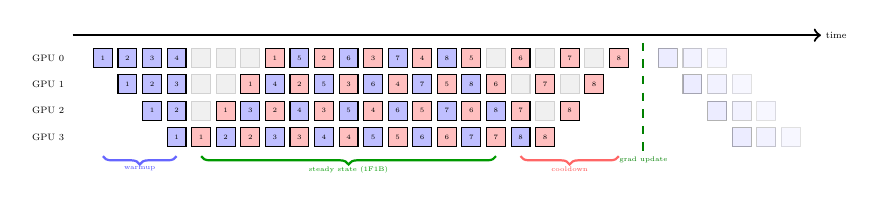
\begin{tikzpicture}[
    scale=0.48, transform shape,
    stage/.style={draw, minimum width=0.50cm, minimum height=0.50cm, font=\tiny, inner sep=1pt},
    fwd/.style={stage, fill=blue!25},
    bwd/.style={stage, fill=red!25},
    bubble/.style={stage, fill=gray!12, draw=gray!35},
  ]
    \def\s{0.65}% step size
    \draw[->, thick] (-0.3, -0.1) -- (19.5, -0.1) node[right, font=\scriptsize] {time};
    \foreach \g in {0,1,2,3} {
      \node[font=\scriptsize, anchor=east] at (-0.4, -\g*0.7 - 0.7) {GPU \g};
    }
    % 1F1B schedule: p=4 stages, m=8 micro-batches, t_f=t_b=1
    % GPU 0: warmup(4F), steady(4×FB), cooldown(4B with bubbles)
    \foreach \t/\sty/\lb in {
      0/fwd/1, 1/fwd/2, 2/fwd/3, 3/fwd/4,
      4/bubble/, 5/bubble/, 6/bubble/,
      7/bwd/1, 8/fwd/5, 9/bwd/2, 10/fwd/6, 11/bwd/3, 12/fwd/7, 13/bwd/4, 14/fwd/8, 15/bwd/5,
      16/bubble/, 17/bwd/6, 18/bubble/, 19/bwd/7, 20/bubble/, 21/bwd/8}
    { \node[\sty] at (\t*\s+0.5, -0.7) {\lb}; }
    % GPU 1: warmup(3F), steady(5×FB), cooldown(3B with bubbles)
    \foreach \t/\sty/\lb in {
      1/fwd/1, 2/fwd/2, 3/fwd/3,
      4/bubble/, 5/bubble/,
      6/bwd/1, 7/fwd/4, 8/bwd/2, 9/fwd/5, 10/bwd/3, 11/fwd/6, 12/bwd/4, 13/fwd/7, 14/bwd/5, 15/fwd/8, 16/bwd/6,
      17/bubble/, 18/bwd/7, 19/bubble/, 20/bwd/8}
    { \node[\sty] at (\t*\s+0.5, -1.4) {\lb}; }
    % GPU 2: warmup(2F), steady(6×FB), cooldown(2B with bubbles)
    \foreach \t/\sty/\lb in {
      2/fwd/1, 3/fwd/2,
      4/bubble/,
      5/bwd/1, 6/fwd/3, 7/bwd/2, 8/fwd/4, 9/bwd/3, 10/fwd/5, 11/bwd/4, 12/fwd/6, 13/bwd/5, 14/fwd/7, 15/bwd/6, 16/fwd/8, 17/bwd/7,
      18/bubble/, 19/bwd/8}
    { \node[\sty] at (\t*\s+0.5, -2.1) {\lb}; }
    % GPU 3: no warmup, all steady (8×FB)
    \foreach \t/\sty/\lb in {
      3/fwd/1, 4/bwd/1, 5/fwd/2, 6/bwd/2, 7/fwd/3, 8/bwd/3, 9/fwd/4, 10/bwd/4,
      11/fwd/5, 12/bwd/5, 13/fwd/6, 14/bwd/6, 15/fwd/7, 16/bwd/7, 17/fwd/8, 18/bwd/8}
    { \node[\sty] at (\t*\s+0.5, -2.8) {\lb}; }
    % Gradient update: vertical bar after last backward (time slot 22)
    \draw[thick, green!50!black, dashed] (22*\s+0.5, -0.3) -- (22*\s+0.5, -3.2)
      node[below, font=\tiny, text=green!50!black] {grad update};
    % Next cycle: faded forward passes starting at time slot 23
    \foreach \col [count=\ci from 0] in {0.30, 0.20, 0.12} {
      \foreach \g in {0,1,2,3} {
        \pgfmathtruncatemacro{\t}{23 + \ci + \g}
        \pgfmathsetmacro{\y}{-\g*0.7 - 0.7}
        \node[fwd, opacity=\col] at (\t*\s+0.5, \y) {};
      }
    }
    % Phase annotations
    \draw[decorate, decoration={brace, mirror, amplitude=3pt}, thick, blue!60]
      (0*\s+0.5, -3.3) -- (3*\s+0.5, -3.3) node[midway, below=4pt, font=\tiny, text=blue!70] {warmup};
    \draw[decorate, decoration={brace, mirror, amplitude=3pt}, thick, green!60!black]
      (4*\s+0.5, -3.3) -- (16*\s+0.5, -3.3) node[midway, below=4pt, font=\tiny, text=green!60!black] {steady state (1F1B)};
    \draw[decorate, decoration={brace, mirror, amplitude=3pt}, thick, red!60]
      (17*\s+0.5, -3.3) -- (21*\s+0.5, -3.3) node[midway, below=4pt, font=\tiny, text=red!70] {cooldown};
  \end{tikzpicture}
  \end{center}

  \vspace{0.2em}
  \begin{columns}
    \begin{column}{0.48\textwidth}
      \textbf{Three phases per GPU:}
      \begin{enumerate}
        \item \textbf{Warmup}: only forward passes fill the pipeline
        \item \textbf{Steady state}: alternate 1 forward, 1 backward
        \item \textbf{Cooldown}: only backward passes drain the pipeline
      \end{enumerate}
    \end{column}
    \begin{column}{0.48\textwidth}
      \textbf{Bubble:} Same as AFAB: $r_{\text{bubble}} = \frac{p-1}{m}$

      \vspace{0.3em}
      \textbf{Key advantage (memory):}
      \begin{itemize}
        \item Only need to store activations for $p$ micro-batches (not $m$!)
        \item Can now safely increase $m \gg p$ to shrink the bubble
      \end{itemize}
    \end{column}
  \end{columns}
\end{frame}

% -----------------------------------------------------------------------
\begin{frame}{1F1B: Scaling Behavior}

  \begin{columns}
    \begin{column}{0.48\textwidth}
      \textbf{Bubble ratio:} $\frac{p-1}{m}$

      \vspace{0.3em}
      \begin{itemize}
        \item Need $m \gg p$ to keep bubble small
        \item But $m$ is constrained by global batch size:\par
          $\text{GBS} = \text{mbs} \times m \times N_{\text{DP}}$
        \item Cannot increase $m$ arbitrarily without growing the batch size (which can hurt convergence)
      \end{itemize}

      \vspace{0.5em}
      \textbf{Cross-node scaling:}
      \begin{itemize}
        \item PP communicates only \emph{activations} between adjacent stages (P2P)
        \item Much less bandwidth-sensitive than TP
        \item Throughput drops only ${\sim}14\%$ going from 1 to 2 nodes, vs.\ ${\sim}43\%$ for TP~\cite{tazi2025ultrascale}
      \end{itemize}
    \end{column}
    \begin{column}{0.48\textwidth}
      \textbf{Bubble ratio for varying $m$ and $p$:}
      \vspace{0.2em}

      \begin{center}
      \begin{tabular}{r | r r r r}
        \toprule
        $p \backslash m$ & 4 & 8 & 16 & 32 \\
        \midrule
        4  & 75\% & 38\% & 19\% & 9\% \\
        8  & --   & 88\% & 44\% & 22\% \\
        16 & --   & --   & 94\% & 47\% \\
        \bottomrule
      \end{tabular}
      \end{center}

      \vspace{0.3em}
      {\small ``--'' means $m < p$ (not enough micro-batches).}

      \vspace{0.5em}
      \begin{alertblock}{Rule of thumb}
        Aim for $m \geq 4p$ for reasonable efficiency ($r_{\text{bubble}} \leq 25\%$).
      \end{alertblock}
    \end{column}
  \end{columns}
\end{frame}

% -----------------------------------------------------------------------
\begin{frame}{Schedule 3: Interleaved 1F1B Layer Distribution}

  \emphdef{Interleaved stages}~\cite{narayanan2021efficient}: assign $v$ \emph{non-contiguous chunks} per GPU.
  A micro-batch loops through all GPUs $v$ times~\cite{narayanan2021efficient}.

  \vspace{0.3em}
  \begin{center}
  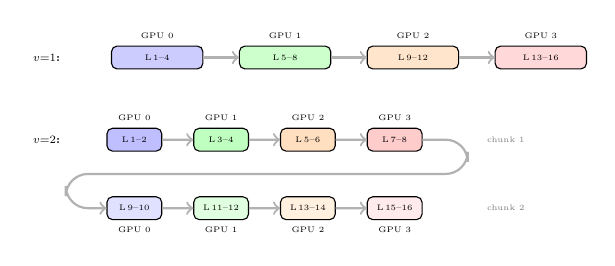
\begin{tikzpicture}[
    scale=0.58, transform shape,
    chunk/.style={draw, rounded corners=2pt, minimum height=0.50cm, font=\tiny, inner sep=2pt},
    gpulbl/.style={font=\scriptsize\bfseries},
    arr/.style={->, thick, gray!60},
    looparr/.style={->, thick, gray!60, rounded corners=4pt},
  ]
    % --- Standard PP (v=1) ---
    \node[gpulbl, anchor=east] at (-0.8, 0) {$v{=}1$:};
    \node[chunk, fill=blue!20,   minimum width=2.0cm] (s0) at (1.2, 0) {L\,1--4};
    \node[chunk, fill=green!20,  minimum width=2.0cm] (s1) at (4.0, 0) {L\,5--8};
    \node[chunk, fill=orange!20, minimum width=2.0cm] (s2) at (6.8, 0) {L\,9--12};
    \node[chunk, fill=red!15,    minimum width=2.0cm] (s3) at (9.6, 0) {L\,13--16};
    \node[font=\tiny, above=1pt] at (s0.north) {GPU 0};
    \node[font=\tiny, above=1pt] at (s1.north) {GPU 1};
    \node[font=\tiny, above=1pt] at (s2.north) {GPU 2};
    \node[font=\tiny, above=1pt] at (s3.north) {GPU 3};
    \draw[arr] (s0) -- (s1);
    \draw[arr] (s1) -- (s2);
    \draw[arr] (s2) -- (s3);

    % --- Interleaved PP (v=2) ---
    \node[gpulbl, anchor=east] at (-0.8, -1.8) {$v{=}2$:};
    % Chunk 1
    \node[chunk, fill=blue!25,   minimum width=1.2cm] (c10) at (0.7, -1.8) {L\,1--2};
    \node[chunk, fill=green!25,  minimum width=1.2cm] (c11) at (2.6, -1.8) {L\,3--4};
    \node[chunk, fill=orange!25, minimum width=1.2cm] (c12) at (4.5, -1.8) {L\,5--6};
    \node[chunk, fill=red!20,    minimum width=1.2cm] (c13) at (6.4, -1.8) {L\,7--8};
    \node[font=\tiny, above=1pt] at (c10.north) {GPU 0};
    \node[font=\tiny, above=1pt] at (c11.north) {GPU 1};
    \node[font=\tiny, above=1pt] at (c12.north) {GPU 2};
    \node[font=\tiny, above=1pt] at (c13.north) {GPU 3};
    \draw[arr] (c10) -- (c11);
    \draw[arr] (c11) -- (c12);
    \draw[arr] (c12) -- (c13);
    % Chunk 2
    \node[chunk, fill=blue!12,   minimum width=1.2cm] (c20) at (0.7, -3.3) {L\,9--10};
    \node[chunk, fill=green!12,  minimum width=1.2cm] (c21) at (2.6, -3.3) {L\,11--12};
    \node[chunk, fill=orange!12, minimum width=1.2cm] (c22) at (4.5, -3.3) {L\,13--14};
    \node[chunk, fill=red!8,     minimum width=1.2cm] (c23) at (6.4, -3.3) {L\,15--16};
    \node[font=\tiny, below=1pt] at (c20.south) {GPU 0};
    \node[font=\tiny, below=1pt] at (c21.south) {GPU 1};
    \node[font=\tiny, below=1pt] at (c22.south) {GPU 2};
    \node[font=\tiny, below=1pt] at (c23.south) {GPU 3};
    \draw[arr] (c20) -- (c21);
    \draw[arr] (c21) -- (c22);
    \draw[arr] (c22) -- (c23);
    % Loop arrow: GPU 3 → right → 180° turn → left between rows → 180° turn → GPU 0
    \draw[arr, rounded corners=8pt]
      (c13.east) -- (8.0,-1.8) -- (8.0,-2.55) -- (-0.8,-2.55) -- (-0.8,-3.3) -- (c20.west);
    % Labels
    \node[font=\tiny, text=gray, anchor=west] at (8.3, -1.8) {chunk 1};
    \node[font=\tiny, text=gray, anchor=west] at (8.3, -3.3) {chunk 2};
  \end{tikzpicture}
  \end{center}

  \vspace{0.2em}
  \begin{columns}
    \begin{column}{0.55\textwidth}
      \textbf{Bubble ratio:}
      $r_{\text{bubble}} = \frac{p - 1}{v \cdot m}$
      : shrinks by factor $v$!

      \vspace{0.2em}
      \textbf{Trade-off:} $v{\times}$ more P2P communication (micro-batch traverses pipeline $v$ times).

      \vspace{0.2em}
      {\small Llama\,3.1 uses interleaved 1F1B~\cite{grattafiori2024llama3}.}
    \end{column}
    \begin{column}{0.42\textwidth}
      {\small
      \begin{tabular}{r r | r}
        \toprule
        $v$ & $m$ & $r_{\text{bubble}}$ \\
        \midrule
        1 & 8 & 88\% \\
        2 & 8 & 44\% \\
        4 & 8 & 22\% \\
        2 & 32 & 11\% \\
        4 & 32 & 5.5\% \\
        \bottomrule
      \end{tabular}
      {\tiny\quad(example $p{=}8$)}}
    \end{column}
  \end{columns}
\end{frame}

% -----------------------------------------------------------------------
\begin{frame}{Interleaved 1F1B: Schedule}

  Each F/B block is $v{\times}$ smaller $\Rightarrow$ pipeline fills/drains faster $\Rightarrow$ smaller bubbles.

  \vspace{0.3em}
  \begin{center}
  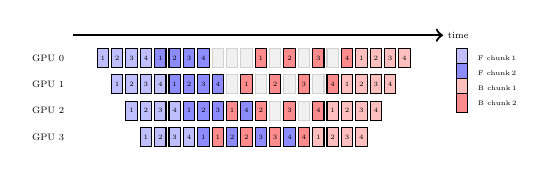
\begin{tikzpicture}[
    scale=0.48, transform shape,
    stage/.style={draw, minimum height=0.50cm, font=\tiny, inner sep=1pt},
    fwd1/.style={stage, fill=blue!25, minimum width=0.30cm},
    bwd1/.style={stage, fill=red!25, minimum width=0.30cm},
    fwd2/.style={stage, fill=blue!45, minimum width=0.30cm},
    bwd2/.style={stage, fill=red!45, minimum width=0.30cm},
    bubble/.style={stage, fill=gray!12, draw=gray!35, minimum width=0.30cm},
  ]
    \def\s{0.38}% half-width step
    \draw[->, thick] (-0.3, -0.1) -- (9.5, -0.1) node[right, font=\scriptsize] {time};
    \foreach \g in {0,1,2,3} {
      \node[font=\scriptsize, anchor=east] at (-0.4, -\g*0.7 - 0.7) {GPU \g};
    }
    % Interleaved 1F1B: p=4, v=2, m=4
    % Virtual pipeline: VS0(GPU0)→VS1(GPU1)→VS2(GPU2)→VS3(GPU3)→VS4(GPU0)→VS5(GPU1)→VS6(GPU2)→VS7(GPU3)
    % fwd1/bwd1 = chunk 1 (lighter), fwd2/bwd2 = chunk 2 (darker)
    %
    % GPU 0 (VS0, VS4): 8F, 3 warmup bubbles, 4B chunk2, 3 cooldown bubbles, 4B chunk1
    \foreach \t/\sty/\lb in {
      0/fwd1/1, 1/fwd1/2, 2/fwd1/3, 3/fwd1/4, 4/fwd2/1, 5/fwd2/2, 6/fwd2/3, 7/fwd2/4,
      8/bubble/, 9/bubble/, 10/bubble/,
      11/bwd2/1, 12/bubble/, 13/bwd2/2, 14/bubble/, 15/bwd2/3, 16/bubble/, 17/bwd2/4,
      18/bwd1/1, 19/bwd1/2, 20/bwd1/3, 21/bwd1/4}
    { \node[\sty] at (\t*\s+0.5, -0.7) {\lb}; }
    % GPU 1 (VS1, VS5): 8F, 2 warmup bubbles, 4B chunk2, 2 cooldown bubbles, 4B chunk1
    \foreach \t/\sty/\lb in {
      1/fwd1/1, 2/fwd1/2, 3/fwd1/3, 4/fwd1/4, 5/fwd2/1, 6/fwd2/2, 7/fwd2/3, 8/fwd2/4,
      9/bubble/, 10/bwd2/1, 11/bubble/, 12/bwd2/2, 13/bubble/, 14/bwd2/3, 15/bubble/, 16/bwd2/4,
      17/bwd1/1, 18/bwd1/2, 19/bwd1/3, 20/bwd1/4}
    { \node[\sty] at (\t*\s+0.5, -1.4) {\lb}; }
    % GPU 2 (VS2, VS6): 8F+1B interleaved, 2 cooldown bubbles, rest B
    \foreach \t/\sty/\lb in {
      2/fwd1/1, 3/fwd1/2, 4/fwd1/3, 5/fwd1/4, 6/fwd2/1, 7/fwd2/2, 8/fwd2/3,
      9/bwd2/1, 10/fwd2/4, 11/bwd2/2, 12/bubble/, 13/bwd2/3, 14/bubble/, 15/bwd2/4,
      16/bwd1/1, 17/bwd1/2, 18/bwd1/3, 19/bwd1/4}
    { \node[\sty] at (\t*\s+0.5, -2.1) {\lb}; }
    % GPU 3 (VS3, VS7): no bubbles, interleaved F/B
    \foreach \t/\sty/\lb in {
      3/fwd1/1, 4/fwd1/2, 5/fwd1/3, 6/fwd1/4, 7/fwd2/1,
      8/bwd2/1, 9/fwd2/2, 10/bwd2/2, 11/fwd2/3, 12/bwd2/3, 13/fwd2/4, 14/bwd2/4,
      15/bwd1/1, 16/bwd1/2, 17/bwd1/3, 18/bwd1/4}
    { \node[\sty] at (\t*\s+0.5, -2.8) {\lb}; }
    % Legend
    \node[fwd1, minimum width=0.28cm] at (10.0, -0.7) {};
    \node[font=\tiny, anchor=west] at (10.3, -0.7) {F chunk\,1};
    \node[fwd2, minimum width=0.28cm] at (10.0, -1.1) {};
    \node[font=\tiny, anchor=west] at (10.3, -1.1) {F chunk\,2};
    \node[bwd1, minimum width=0.28cm] at (10.0, -1.5) {};
    \node[font=\tiny, anchor=west] at (10.3, -1.5) {B chunk\,1};
    \node[bwd2, minimum width=0.28cm] at (10.0, -1.9) {};
    \node[font=\tiny, anchor=west] at (10.3, -1.9) {B chunk\,2};
  \end{tikzpicture}
  \end{center}

  \vspace{0.2em}
  \begin{columns}
    \begin{column}{0.48\textwidth}
      With $v{=}2$, $p{=}4$, $m{=}4$:
      \begin{itemize}
        \item Each block is $\frac{1}{v}$ the size
        \item Virtual pipeline depth: $v \cdot p = 8$
        \item Bubble ratio: $\frac{p-1}{v \cdot m} = \frac{3}{8} = 37.5\%$
      \end{itemize}
    \end{column}
    \begin{column}{0.48\textwidth}
      Compare to standard 1F1B:
      \begin{itemize}
        \item Same $m{=}4$: bubble $\frac{3}{4} = 75\%$
        \item $v{=}2$ \textbf{halves} the bubble
        \item But $2{\times}$ P2P communication volume
      \end{itemize}
    \end{column}
  \end{columns}
\end{frame}

% -----------------------------------------------------------------------
\begin{frame}{Interleaved 1F1B: Depth-First vs.\ Breadth-First}

  With interleaved stages, a scheduling choice arises: which micro-batch/chunk to run next on a given GPU?

  \vspace{0.5em}
  \begin{columns}
    \begin{column}{0.48\textwidth}
      \textbf{Depth-first}~\cite{lamy2023breadthfirst}
      \begin{itemize}
        \item Prioritize advancing \emph{earlier} micro-batches through \emph{later} chunks
        \item Gets micro-batches out of the pipeline faster
        \item Backward starts sooner $\Rightarrow$ \emph{less activation memory}
        \item Can reduce peak memory significantly
      \end{itemize}
    \end{column}
    \begin{column}{0.48\textwidth}
      \textbf{Breadth-first}~\cite{lamy2023breadthfirst}
      \begin{itemize}
        \item Prioritize injecting \emph{new} micro-batches into \emph{early} chunks
        \item Fills the pipeline more aggressively
        \item Can achieve slightly \emph{better throughput}
        \item But keeps more activations alive simultaneously
      \end{itemize}
    \end{column}
  \end{columns}

  \vspace{0.5em}
  \begin{alertblock}{In practice}
    The optimal choice depends on memory constraints and pipeline depth. Llama\,3.1 uses a tunable priority between depth-first and breadth-first scheduling~\cite{grattafiori2024llama3}.
  \end{alertblock}
\end{frame}

% -----------------------------------------------------------------------
\begin{frame}{Schedule 4: Zero Bubble}

  Can we \emph{eliminate} the bubble entirely? Key insight from~\cite{qi2023zero}: decompose the backward pass.

  \vspace{0.3em}
  \begin{columns}
    \begin{column}{0.55\textwidth}
      \textbf{Backward pass has two independent parts:}
      \begin{description}[labelwidth=0.6cm]
        \item[\textbf{B}] Backward for \emph{inputs} (compute $\frac{\partial \mathcal{L}}{\partial x}$)\par
          Needed by the previous stage immediately
        \item[\textbf{W}] Backward for \emph{weights} (compute $\frac{\partial \mathcal{L}}{\partial \theta}$)\par
          Only needed before the optimizer step
      \end{description}

      \vspace{0.3em}
      $\Rightarrow$ \textbf{W can be deferred} and scheduled flexibly to \emph{fill bubble slots}!

      \vspace{0.3em}
      \textbf{ZB-H1:} Schedule W operations in cooldown bubbles.\par
      \textbf{ZB-H2:} Use ILP solver to find a schedule with \emph{zero bubble} (in theory).
    \end{column}
    \begin{column}{0.42\textwidth}
      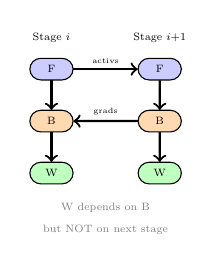
\begin{tikzpicture}[
        scale=0.55, transform shape,
        node distance=0.8cm and 1.2cm,
        op/.style={draw, rounded corners, minimum width=1.0cm, minimum height=0.5cm, font=\scriptsize},
      ]
        % Computation graph
        \node[op, fill=blue!20] (f1) at (0, 0) {F};
        \node[op, fill=blue!20] (f2) at (2.5, 0) {F};
        \node[op, fill=orange!30] (b1) at (0, -1.2) {B};
        \node[op, fill=orange!30] (b2) at (2.5, -1.2) {B};
        \node[op, fill=green!25] (w1) at (0, -2.4) {W};
        \node[op, fill=green!25] (w2) at (2.5, -2.4) {W};

        \draw[->, thick] (f1) -- (f2) node[midway, above, font=\tiny] {activs};
        \draw[->, thick] (f1) -- (b1);
        \draw[->, thick] (f2) -- (b2);
        \draw[->, thick] (b2) -- (b1) node[midway, above, font=\tiny] {grads};
        \draw[->, thick] (b1) -- (w1);
        \draw[->, thick] (b2) -- (w2);

        \node[font=\scriptsize, gray] at (1.25, -3.2) {W depends on B};
        \node[font=\scriptsize, gray] at (1.25, -3.7) {but NOT on next stage};

        % Stage labels
        \node[font=\scriptsize, anchor=south] at (0, 0.5) {Stage $i$};
        \node[font=\scriptsize, anchor=south] at (2.5, 0.5) {Stage $i{+}1$};
      \end{tikzpicture}
    \end{column}
  \end{columns}

  \vspace{0.3em}
  \textbf{Optimization:} Measure $t_F, t_B, t_W$ for each stage, then solve an Integer Linear Program to minimize total idle time~\cite{qi2023zero}.
\end{frame}

% -----------------------------------------------------------------------
\begin{frame}{Zero Bubble: Schedules Comparison}

  \begin{center}
  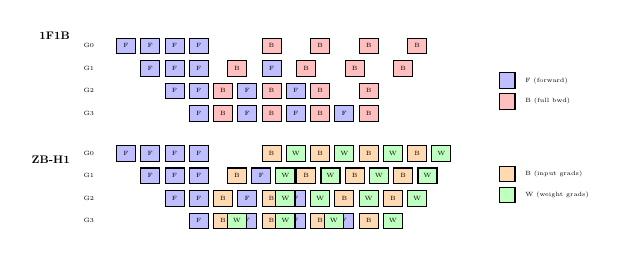
\begin{tikzpicture}[
    scale=0.44, transform shape,
    cell/.style={draw, minimum width=0.55cm, minimum height=0.45cm, font=\tiny, inner sep=0.5pt},
    fwd/.style={cell, fill=blue!25},
    bfull/.style={cell, fill=red!25},
    binp/.style={cell, fill=orange!30},
    bwt/.style={cell, fill=green!25},
    bubble/.style={cell, fill=gray!10, draw=gray!30},
  ]
    % === 1F1B (coarse backward) ===
    \node[font=\small, anchor=east] at (-1.0, 0.3) {\textbf{1F1B}};
    \foreach \g in {0,1,2,3} {
      \node[font=\tiny, anchor=east] at (-0.3, -\g*0.65) {G\g};
    }
    % GPU 0: F F F F _ B _ B _ B _ B
    \node[fwd] at (0.5, 0) {F};
    \node[fwd] at (1.2, 0) {F};
    \node[fwd] at (1.9, 0) {F};
    \node[fwd] at (2.6, 0) {F};
    \node[bfull] at (4.7, 0) {B};
    \node[bfull] at (6.1, 0) {B};
    \node[bfull] at (7.5, 0) {B};
    \node[bfull] at (8.9, 0) {B};

    % GPU 1
    \node[fwd] at (1.2, -0.65) {F};
    \node[fwd] at (1.9, -0.65) {F};
    \node[fwd] at (2.6, -0.65) {F};
    \node[bfull] at (3.7, -0.65) {B};
    \node[fwd] at (4.7, -0.65) {F};
    \node[bfull] at (5.7, -0.65) {B};
    \node[bfull] at (7.1, -0.65) {B};
    \node[bfull] at (8.5, -0.65) {B};

    % GPU 2
    \node[fwd] at (1.9, -1.3) {F};
    \node[fwd] at (2.6, -1.3) {F};
    \node[bfull] at (3.3, -1.3) {B};
    \node[fwd] at (4.0, -1.3) {F};
    \node[bfull] at (4.7, -1.3) {B};
    \node[fwd] at (5.4, -1.3) {F};
    \node[bfull] at (6.1, -1.3) {B};
    \node[bfull] at (7.5, -1.3) {B};

    % GPU 3
    \node[fwd] at (2.6, -1.95) {F};
    \node[bfull] at (3.3, -1.95) {B};
    \node[fwd] at (4.0, -1.95) {F};
    \node[bfull] at (4.7, -1.95) {B};
    \node[fwd] at (5.4, -1.95) {F};
    \node[bfull] at (6.1, -1.95) {B};
    \node[fwd] at (6.8, -1.95) {F};
    \node[bfull] at (7.5, -1.95) {B};

    % === ZB-H1 (split B and W) ===
    \node[font=\small, anchor=east] at (-1.0, -3.3) {\textbf{ZB-H1}};
    \foreach \g in {0,1,2,3} {
      \node[font=\tiny, anchor=east] at (-0.3, -\g*0.65 - 3.1) {G\g};
    }
    % GPU 0
    \node[fwd] at (0.5, -3.1) {F};
    \node[fwd] at (1.2, -3.1) {F};
    \node[fwd] at (1.9, -3.1) {F};
    \node[fwd] at (2.6, -3.1) {F};
    \node[binp] at (4.7, -3.1) {B};
    \node[bwt] at (5.4, -3.1) {W};
    \node[binp] at (6.1, -3.1) {B};
    \node[bwt] at (6.8, -3.1) {W};
    \node[binp] at (7.5, -3.1) {B};
    \node[bwt] at (8.2, -3.1) {W};
    \node[binp] at (8.9, -3.1) {B};
    \node[bwt] at (9.6, -3.1) {W};

    % GPU 1
    \node[fwd] at (1.2, -3.75) {F};
    \node[fwd] at (1.9, -3.75) {F};
    \node[fwd] at (2.6, -3.75) {F};
    \node[binp] at (3.7, -3.75) {B};
    \node[fwd] at (4.4, -3.75) {F};
    \node[bwt] at (5.1, -3.75) {W};
    \node[binp] at (5.7, -3.75) {B};
    \node[bwt] at (6.4, -3.75) {W};
    \node[binp] at (7.1, -3.75) {B};
    \node[bwt] at (7.8, -3.75) {W};
    \node[binp] at (8.5, -3.75) {B};
    \node[bwt] at (9.2, -3.75) {W};

    % GPU 2
    \node[fwd] at (1.9, -4.4) {F};
    \node[fwd] at (2.6, -4.4) {F};
    \node[binp] at (3.3, -4.4) {B};
    \node[fwd] at (4.0, -4.4) {F};
    \node[binp] at (4.7, -4.4) {B};
    \node[fwd] at (5.4, -4.4) {F};
    \node[bwt] at (6.1, -4.4) {W};
    \node[binp] at (6.8, -4.4) {B};
    \node[bwt] at (7.5, -4.4) {W};
    \node[binp] at (8.2, -4.4) {B};
    \node[bwt] at (8.9, -4.4) {W};
    \node[bwt] at (5.1, -4.4) {W};

    % GPU 3
    \node[fwd] at (2.6, -5.05) {F};
    \node[binp] at (3.3, -5.05) {B};
    \node[fwd] at (4.0, -5.05) {F};
    \node[binp] at (4.7, -5.05) {B};
    \node[fwd] at (5.4, -5.05) {F};
    \node[binp] at (6.1, -5.05) {B};
    \node[fwd] at (6.8, -5.05) {F};
    \node[binp] at (7.5, -5.05) {B};
    \node[bwt] at (3.7, -5.05) {W};
    \node[bwt] at (5.1, -5.05) {W};
    \node[bwt] at (6.5, -5.05) {W};
    \node[bwt] at (8.2, -5.05) {W};

    % Legend
    \node[fwd, minimum width=0.45cm] at (11.5, -1.0) {};
    \node[font=\tiny, anchor=west] at (11.9, -1.0) {F (forward)};
    \node[bfull, minimum width=0.45cm] at (11.5, -1.6) {};
    \node[font=\tiny, anchor=west] at (11.9, -1.6) {B (full bwd)};
    \node[binp, minimum width=0.45cm] at (11.5, -3.7) {};
    \node[font=\tiny, anchor=west] at (11.9, -3.7) {B (input grads)};
    \node[bwt, minimum width=0.45cm] at (11.5, -4.3) {};
    \node[font=\tiny, anchor=west] at (11.9, -4.3) {W (weight grads)};
  \end{tikzpicture}
  \end{center}

  \vspace{0.2em}
  \begin{itemize}
    \item \textbf{1F1B}: Backward is monolithic $\Rightarrow$ rigid scheduling, bubbles in warmup/cooldown
    \item \textbf{ZB-H1}: Split into B + W, schedule W flexibly $\Rightarrow$ fills cooldown bubbles
    \item \textbf{ZB-H2}: ILP-optimized placement of F, B, W $\Rightarrow$ \emph{theoretically zero bubble}
  \end{itemize}
\end{frame}

% -----------------------------------------------------------------------
\begin{frame}{DualPipe (DeepSeek-V3)}

  \emphdef{DualPipe}~\cite{deepseekai2024deepseekv3}: extends zero-bubble ideas with \emph{bidirectional} pipeline streams.

  \vspace{0.3em}
  \begin{columns}
    \begin{column}{0.55\textwidth}
      \textbf{Key ideas:}
      \begin{enumerate}
        \item Split backward into B (input grads) and W (weight grads), as in Zero Bubble
        \item Run \textbf{two streams} propagating from \emph{both ends} of the pipeline simultaneously
        \item Interleave the two streams to keep all GPUs busy
        \item Overlap computation and all-to-all communication
      \end{enumerate}

      \vspace{0.3em}
      \textbf{Result:} Near-zero pipeline bubble with minimal additional communication overhead.

      \vspace{0.3em}
      DeepSeek-V3 reports \emph{``near-zero all-to-all communication overhead''} with this schedule.
    \end{column}
    \begin{column}{0.42\textwidth}
      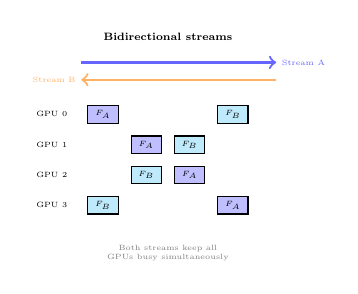
\begin{tikzpicture}[
        scale=0.55, transform shape,
        cell/.style={draw, minimum width=0.7cm, minimum height=0.4cm, font=\tiny, inner sep=0.5pt},
        fwdA/.style={cell, fill=blue!25},
        fwdB/.style={cell, fill=cyan!25},
        bwdA/.style={cell, fill=red!20},
        bwdB/.style={cell, fill=orange!25},
      ]
        \node[font=\scriptsize] at (2.0, 1.0) {\textbf{Bidirectional streams}};

        % Stream A: left to right
        \draw[->, thick, blue!60] (0, 0.4) -- (4.5, 0.4) node[right, font=\tiny] {Stream A};
        % Stream B: right to left
        \draw[->, thick, orange!60] (4.5, 0.0) -- (0, 0.0) node[left, font=\tiny] {Stream B};

        % GPUs
        \foreach \g in {0,1,2,3} {
          \node[font=\tiny, anchor=east] at (-0.2, -\g*0.7 - 0.8) {GPU \g};
        }

        % Stream A forwards (left to right)
        \node[fwdA] at (0.5, -0.8) {$F_A$};
        \node[fwdA] at (1.5, -1.5) {$F_A$};
        \node[fwdA] at (2.5, -2.2) {$F_A$};
        \node[fwdA] at (3.5, -2.9) {$F_A$};

        % Stream B forwards (right to left)
        \node[fwdB] at (3.5, -0.8) {$F_B$};
        \node[fwdB] at (2.5, -1.5) {$F_B$};
        \node[fwdB] at (1.5, -2.2) {$F_B$};
        \node[fwdB] at (0.5, -2.9) {$F_B$};

        % Overlap annotation
        \node[font=\tiny, gray, text width=3cm, align=center] at (2.0, -4.0) {Both streams keep all GPUs busy simultaneously};
      \end{tikzpicture}
    \end{column}
  \end{columns}

  \vspace{0.3em}
  \begin{alertblock}{Complexity}
    DualPipe requires careful measurement of per-operation timings and sophisticated scheduling.
    Practical implementations use heuristics or ILP solvers to find near-optimal schedules.
  \end{alertblock}
\end{frame}

% -----------------------------------------------------------------------
\begin{frame}{PP Schedules: Summary}

  \begin{center}
  \renewcommand{\arraystretch}{1.2}
  \begin{tabular}{l c c c}
    \toprule
    \textbf{Schedule} & \textbf{Bubble ratio} & \textbf{Peak activation memory} & \textbf{Extra comm.} \\
    \midrule
    AFAB (GPipe) & $\frac{p-1}{m}$ & $O(m)$ micro-batches & $1\times$ \\[0.3em]
    1F1B         & $\frac{p-1}{m}$ & $O(p)$ micro-batches & $1\times$ \\[0.3em]
    Interleaved 1F1B & $\frac{p-1}{v \cdot m}$ & $O(p)$ micro-batches & $v\times$ \\[0.3em]
    Zero Bubble  & $\to 0$ (ILP) & $O(p)$ micro-batches & $1\times$ \\[0.3em]
    DualPipe     & $\approx 0$ & $O(p)$ micro-batches & ${\sim}1\times$ \\
    \bottomrule
  \end{tabular}
  \end{center}

  \vspace{0.3em}
  \textbf{Historical progression:}
  \begin{itemize}
    \item GPipe $\to$ 1F1B / PipeDream $\to$ Interleaved $\to$ Zero Bubble $\to$ DualPipe
    \item Each step either reduces the bubble or reduces memory, at increasing implementation complexity
  \end{itemize}

  \vspace{0.3em}
  \begin{alertblock}{PP vs.\ ZeRO-3}
    Both solve ``model doesn't fit on one GPU'' but differently: PP transfers \emph{activations} between stages; ZeRO-3 transfers \emph{weights}. PP prefers large \texttt{grad\_acc} to hide the bubble; ZeRO-3 prefers large \texttt{mbs} and \texttt{seq\_len} to hide communication.
    In practice, PP combines well with ZeRO-1/2 (e.g.\ DeepSeek-V3 uses PP + ZeRO-1).
  \end{alertblock}
\end{frame}
